% This LaTeX document needs to be compiled with XeLaTeX.
\documentclass[10pt]{article}
\usepackage[utf8]{inputenc}
\usepackage{graphicx}
\usepackage[export]{adjustbox}
\graphicspath{ {./images/} }
\usepackage{amsmath}
\usepackage{amsfonts}
\usepackage{amssymb}
\usepackage[version=4]{mhchem}
\usepackage{stmaryrd}
\usepackage[fallback]{xeCJK}
\usepackage{polyglossia}
\usepackage{fontspec}
\setCJKmainfont{Noto Serif CJK TC}

\setmainlanguage{polish}
\setmainfont{CMU Serif}

\title{ARKUSZ PRÓBNEJ MATURY Z OPERONEM MATEMATYKA }

\author{}
\date{}


\begin{document}
\maketitle
\section*{POZIOM PODSTAWOWY}
\section*{Czas pracy: 170 minut}
\section*{Instrukcja dla zdającego}
\begin{enumerate}
  \item Sprawdź, czy arkusz egzaminacyjny zawiera 15 stron (zadania 1.-34.). Ewentualny brak zgłoś przewodniczącemu zespołu nadzorującego egzamin.
  \item Rozwiązania zadań i odpowiedzi zapisz w miejscu na to przeznaczonym.
  \item W zadaniach zamkniętych (1.-25.) zaznacz jedną poprawną odpowiedź.
  \item W rozwiązaniach zadań otwartych (26.-34.) przedstaw tok rozumowania prowadzący do ostatecznego wyniku.
  \item Pisz czytelnie. Używaj długopisu/pióra tylko z czarnym tuszem/atramentem.
  \item Nie używaj korektora, a błędne zapisy wyraźnie przekreśl.
  \item Zapisy w brudnopisie nie będą oceniane.
  \item Obok numeru każdego zadania podana jest maksymalna liczba punktów możliwych do uzyskania.
  \item Możesz korzystać z zestawu wzorów matematycznych, cyrkla i linijki oraz kalkulatora.
\end{enumerate}

\section*{Życzymy powodzenia!}
Za rozwiązanie wszystkich zadań można otrzymać łącznie 50 punktów.\\
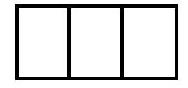
\includegraphics[max width=\textwidth, center]{2024_11_21_6574e892c2387ce90f12g-01(1)}

KOD\\
ZDAJĄCEGO

PESEL ZDAJĄCEGO

LISTOPAD\\
2020

Wpisuje zdający przed rozpoczęciem pracy\\
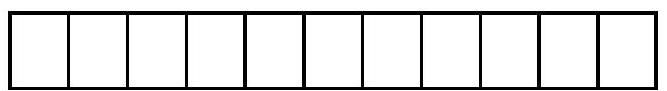
\includegraphics[max width=\textwidth, center]{2024_11_21_6574e892c2387ce90f12g-01}

\section*{ZADANIA ZAMKNIĘTE}
\section*{W zadaniach 1.-25. wybierz i zaznacz jedną poprawną odpowiedź.}
\section*{Zadanie 1. (0-1)}
Liczbą odwrotną do liczby \(\frac{\left(\frac{1}{2}\right)^{-1}-5}{2^{-2}-\left(\frac{2}{3}\right)^{-2}}\) jest:\\
A. \(\frac{2}{3}\)\\
B. \(-\frac{2}{3}\)\\
C. \(1 \frac{1}{2}\)\\
D. \(-1 \frac{1}{2}\)

\section*{Zadanie 2. (0-1)}
Przedział liczbowy \(\langle 2,7\rangle\) jest iloczynem zbioru \(A=\langle m, \infty)\) i zbioru \(B=(-3,7\rangle\) dla \(m\) równego:\\
A. 7\\
B. 2\\
C. -3\\
D. -1

\section*{Zadanie 3. (0-1)}
Liczba dodatnia \(a\) jest zapisana w postaci ułamka zwykłego. Licznik tego ułamka zwiększono o 20\%, a jego mianownik zmniejszono o 20\%. Otrzymano w ten sposób liczbę \(b\), taką, że:\\
A. \(b=a\)\\
B. \(b=\frac{2}{3} a\)\\
C. \(b=0,4 a\)\\
D. \(b=1,5 a\)

\section*{Zadanie 4. (0-1)}
W rozwinięciu dziesiętnym ułamka \(\frac{5}{7}\) na setnym miejscu po przecinku stoi cyfra:\\
A. 7\\
B. 1\\
C. 2\\
D. 5

\section*{Zadanie 5. (0-1)}
Wartość wyrażenia \(|8-4 \sqrt{5}|-(3 \sqrt{5}-8)\) jest równa:\\
A. \(\sqrt{5}\)\\
B. \(7 \sqrt{5}+16\)\\
C. 16\\
D. \(16-7 \sqrt{5}\)

\section*{Zadanie 6. (0-1)}
Jeżeli \(\log 5=a\) i \(\log 3=b\), to \(\log 15\) jest równy:\\
A. \(a b\)\\
B. \(\frac{a}{b}\)\\
C. \(a+b\)\\
D. \(a-b\)

\section*{Zadanie 7. (0-1)}
Stosunek pól dwóch trójkątów równobocznych wynosi \(\frac{9}{16}\), a długość boku większego trójkąta jest równa 12 cm . Mniejszy trójkąt ma bok długości:\\
A. \(6,75 \mathrm{~cm}\)\\
B. \(21 \frac{1}{3} \mathrm{~cm}\)\\
C. 16 cm\\
D. 9 cm

\section*{BRUDNOPIS (nie podlega ocenie)}
\begin{center}

\includegraphics[max width=\textwidth]{2024_11_21_6574e892c2387ce90f12g-03}
\end{center}

\section*{Zadanie 8. (0-1)}
Punkt \(S\) jest środkiem boku kwadratu \(A B C D\), a długość odcinka \(A S\) wynosi 5 cm . Obwód trójkąta \(A D S\) jest równy:\\
A. \((5+2 \sqrt{5}) \mathrm{cm}\)\\
B. \((10+2 \sqrt{5}) \mathrm{cm}\)\\
C. \((5+\sqrt{5}) \mathrm{cm}\)\\
D. \((10+\sqrt{5}) \mathrm{cm}\)\\
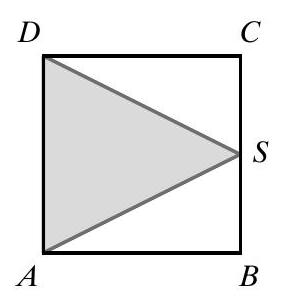
\includegraphics[max width=\textwidth, center]{2024_11_21_6574e892c2387ce90f12g-04(1)}

\section*{Zadanie 9. (0-1)}
Prosta \(A B\) jest styczna w punkcie \(B\) do okręgu o środku \(O\) (patrz rysunek).\\
Miara kąta \(A C B\) jest równa:\\
A. \(90^{\circ}\)\\
B. \(32^{\circ}\)\\
C. \(58^{\circ}\)\\
D. \(29^{\circ}\)\\
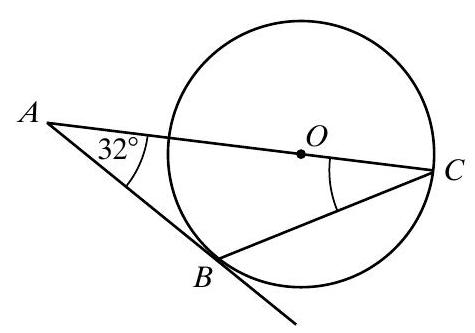
\includegraphics[max width=\textwidth, center]{2024_11_21_6574e892c2387ce90f12g-04}

Zadanie 10. (0-1)\\
Punkty \(A=(1,2)\) i \(B=(-3,5)\) są dwoma wierzchołkami kwadratu \(A B C D\). Obwód tego kwadratu jest równy:\\
A. 5\\
B. 20\\
C. 25\\
D. \(4 \sqrt{13}\)

\section*{Zadanie 11. (0-1)}
Wartości ujemnych nie przyjmuje funkcja \(f\) określona wzorem:\\
A. \(f(x)=-x^{2}+1\)\\
B. \(f(x)=x^{2}-1\)\\
C. \(f(x)=-x^{2}-1\)\\
D. \(f(x)=x^{2}+1\)

\section*{Zadanie 12. (0-1)}
Prosta będąca wykresem funkcji \(f(x)=a x+b\) przechodzi tylko przez I, II i IV ćwiartkę układu współrzędnych. Wynika stąd, że:\\
A. \(a>0 \mathrm{i} b>0\)\\
B. \(a<0 \mathrm{i} b>0\)\\
C. \(a>0\) i \(b<0\)\\
D. \(a<0 \mathrm{i} b<0\)

\section*{Zadanie 13. (0-1)}
Wspólnym pierwiastkiem równania \(3 x\left(x+\frac{2}{3}\right)(2 x-5)=0\) oraz równania \(\frac{2 x-5}{3 x+2}=0\) jest liczba:\\
A. \(\frac{2}{3}\)\\
B. \(-\frac{2}{3}\)\\
C. 2,5\\
D. \(-2,5\)

\section*{Zadanie 14. (0-1)}
Jeżeli sinus kąta ostrego \(\alpha\) wynosi \(\frac{2 \sqrt{3}}{5}\), to wartość tangensa kąta ostrego \(\alpha\) jest równa:\\
A. \(\frac{2 \sqrt{39}}{13}\)\\
B. \(\frac{\sqrt{13}}{5}\)\\
C. \(\frac{\sqrt{39}}{6}\)\\
D. \(\frac{5 \sqrt{13}}{13}\)

\section*{BRUDNOPIS (nie podlega ocenie)}
\begin{center}

\includegraphics[max width=\textwidth]{2024_11_21_6574e892c2387ce90f12g-05}
\end{center}

\section*{Zadanie 15. (0-1)}
Trzecim wyrazem ciągu geometrycznego jest liczba 3, a szóstym jest liczba - 24. Suma czterech początkowych wyrazów tego ciągu wynosi:\\
A. \(11 \frac{1}{4}\)\\
B. \(3 \frac{3}{4}\)\\
C. \(-3 \frac{3}{4}\)\\
D. \(-11 \frac{1}{4}\)

\section*{Zadanie 16. (0-1)}
Jeśli nieskończony ciąg \(\left(a_{n}\right)\) jest ciągiem arytmetycznym, w którym \(a_{1}=5\) i różnica \(r=-3\), to:\\
A. \(a_{n}=2-3 n\)\\
B. \(a_{n}=8-3 n\)\\
C. \(a_{n}=-8-3 n\)\\
D. \(a_{n}=3+3 n\)

\section*{Zadanie 17. (0-1)}
Największą liczbą naturalną, która nie spełnia nierówności \(32^{10}-2^{48} \cdot x+8 \cdot 4^{23} \leq\left(64^{4}\right)^{2}\), jest liczba:\\
A. \(2^{48}\)\\
B. 6\\
C. 5\\
D. 4

\section*{Zadanie 18. (0-1)}
Na rysunku przedstawiono wykres funkcji \(f\).\\
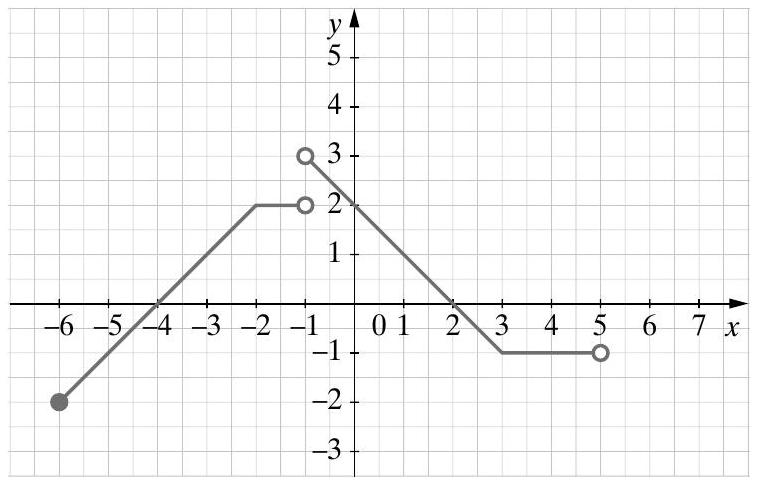
\includegraphics[max width=\textwidth, center]{2024_11_21_6574e892c2387ce90f12g-06}

Dziedziną funkcji \(f\) jest:\\
A. \(\langle-6,5) \backslash\{-1\}\)\\
B. \(\langle-6,5\rangle \backslash\{-1\}\)\\
C. \((-6,-1) \cup(-1,5)\)\\
D. \(\langle-6,5)\)

\section*{Zadanie 19. (0-1)}
Proste o równaniach \(y=(2 m+1) x-4\) i \(y=(6-3 m) x+4\) są równoległe wtedy, gdy:\\
A. \(m=-1\)\\
B. \(m=-3\)\\
C. \(m=1\)\\
D. \(m=3\)

\section*{Zadanie 20. (0-1)}
Funkcja kwadratowa, której miejscami zerowymi są liczby -2 i 4 oraz do której należy punkt o współrzędnych \((0,8)\), jest określona wzorem:\\
A. \(f(x)=-(x-2)(x+4)\)\\
B. \(f(x)=(x-2)(x+4)\)\\
C. \(f(x)=(x+2)(x-4)\)\\
D. \(f(x)=-(x+2)(x-4)\)

\section*{BRUDNOPIS (nie podlega ocenie)}
\begin{center}

\includegraphics[max width=\textwidth]{2024_11_21_6574e892c2387ce90f12g-07}
\end{center}

\section*{Zadanie 21. (0-1)}
W turnieju bilardowym, w którym zawodnicy grali każdy z każdym, rozegrano 28 partii. Liczba zawodników biorących udział w tym turnieju wynosi:\\
A. 6\\
B. 7\\
C. 8\\
D. 9

\section*{Zadanie 22. (0-1)}
W trójkącie \(A B C\) o polu równym \(10 \mathrm{~cm}^{2}\) długość boku \(A B\) wynosi 5 cm , a kąt przy wierzchołku \(A\) ma miarę \(45^{\circ}\). Długość boku \(A C\) jest równa:\\
A. \(2 \sqrt{2} \mathrm{~cm}\)\\
B. \(4 \sqrt{2} \mathrm{~cm}\)\\
C. 4 cm\\
D. 2 cm

\section*{Zadanie 23. (0-1)}
Liczba wierzchołków pewnego ostrosłupa jest o 5 mniejsza od liczby krawędzi. Podstawą tego ostrosłupa jest:\\
A. siedmiokąt\\
B. ośmiokąt\\
C. pięciokąt\\
D. sześciokąt

\section*{Zadanie 24. (0-1)}
Przekątna przekroju osiowego walca ma długości 4 cm i jest nachylona do płaszczyzny podstawy pod kątem \(60^{\circ}\). Obwód podstawy tego walca jest równy:\\
A. \(4 \pi \mathrm{~cm}\)\\
B. \(2 \sqrt{3} \pi \mathrm{~cm}\)\\
C. \(2 \pi \mathrm{~cm}\)\\
D. \(\pi \mathrm{cm}\)

\section*{Zadanie 25. (0-1)}
Ze zbioru liczb \(1,8,2,8,4,8,6\) usunięto jedną liczbę w ten sposób, że mediana otrzymanego zbioru liczb zmniejszyła się o 1 . Wynika stąd, że usunięto liczbę:\\
A. 1\\
B. 8\\
C. 2\\
D. 6

\section*{BRUDNOPIS (nie podlega ocenie)}
\begin{center}

\includegraphics[max width=\textwidth]{2024_11_21_6574e892c2387ce90f12g-09}
\end{center}

\section*{ZADANIA OTWARTE}
Rozwiązania zadań 26.-34. należy zapisać w wyznaczonych miejscach pod treścią zadania.

\section*{Zadanie 26. (0-2)}
Oblicz wartość parametru \(m\), dla którego miejscem zerowym funkcji \(f(x)=\frac{5-2 m}{2} x+2\) jest liczba 4.\\

\includegraphics[max width=\textwidth, center]{2024_11_21_6574e892c2387ce90f12g-10}

Odpowiedź: \(\qquad\)

\section*{Zadanie 27. (0-2)}
Punkty \(A=(2,5), B=(0,7), C=(-4,5)\) są trzema kolejnymi wierzchołkami równoległoboku \(A B C D\). Oblicz współrzędne wierzchołka \(D\) tego równoległoboku.

\begin{center}
\begin{tabular}{|c|c|c|c|c|c|c|c|c|c|c|c|c|c|c|c|c|c|c|c|c|c|c|c|c|c|c|c|c|c|}
\hline
 &  &  &  &  &  &  &  &  &  &  &  &  &  &  &  &  &  &  &  &  &  &  &  &  &  &  &  &  &  \\
\hline
 &  &  &  &  &  &  &  &  &  &  &  &  &  &  &  &  &  &  &  &  &  &  &  &  &  &  &  &  &  \\
\hline
 &  &  &  &  &  &  &  &  &  &  &  &  &  &  &  &  &  &  &  &  &  &  &  &  &  &  &  &  &  \\
\hline
 &  &  &  &  &  &  &  &  &  &  &  &  &  &  &  &  &  &  &  &  &  &  &  &  &  &  &  &  &  \\
\hline
 &  &  &  &  &  &  &  &  &  &  &  &  &  &  &  &  &  &  &  &  &  &  &  &  &  &  &  &  &  \\
\hline
 &  &  &  &  &  &  &  &  &  &  &  &  &  &  &  &  &  &  &  &  &  &  &  &  &  &  &  &  &  \\
\hline
 &  &  &  &  &  &  &  &  &  &  &  &  &  &  &  &  &  &  &  &  &  &  &  &  &  &  &  &  &  \\
\hline
 &  &  &  &  &  &  &  &  &  &  &  &  &  &  &  &  &  &  &  &  &  &  &  &  &  &  &  &  &  \\
\hline
 &  &  &  &  &  &  &  &  &  &  &  &  &  &  &  &  &  &  &  &  &  &  &  &  &  &  &  &  &  \\
\hline
 & - &  &  &  &  &  &  &  &  &  &  &  &  &  &  &  &  &  &  &  &  &  &  &  &  &  &  &  &  \\
\hline
 &  &  &  &  &  &  &  &  &  &  &  &  &  &  &  &  &  &  &  &  &  &  &  &  &  &  &  &  &  \\
\hline
 &  &  &  &  &  &  &  &  &  &  &  &  &  &  &  &  &  &  &  &  &  &  &  &  &  &  &  &  &  \\
\hline
 &  &  &  &  &  &  &  &  &  &  &  &  &  &  &  &  &  &  &  &  &  &  &  &  &  &  &  &  &  \\
\hline
 &  &  &  &  &  &  &  &  &  &  &  &  &  &  &  &  &  &  &  &  &  &  &  &  &  &  &  &  &  \\
\hline
\end{tabular}
\end{center}

\section*{Zadanie 28. (0-2)}
Wartość wyrażenia \(\frac{\operatorname{tg} 30^{\circ} \cdot \operatorname{tg} 60^{\circ}-4 \sin ^{2} 60^{\circ}}{\cos ^{2} 40^{\circ}+\cos ^{2} 50^{\circ}}\) sprowadź do najprostszej postaci.

\begin{center}
\begin{tabular}{|c|c|c|c|c|c|c|c|c|c|c|c|c|c|c|c|c|c|c|c|c|c|c|c|}
\hline
 &  &  &  &  &  &  &  &  &  &  &  &  &  &  &  &  &  &  &  &  &  &  &  \\
\hline
 &  &  &  &  &  &  &  &  &  &  &  &  &  &  &  &  &  &  &  &  &  &  &  \\
\hline
 &  &  &  &  &  &  &  &  &  &  &  &  &  &  &  &  &  &  &  &  &  &  &  \\
\hline
 &  &  &  &  &  &  &  &  &  &  &  &  &  &  &  &  &  &  &  &  &  &  &  \\
\hline
 &  &  &  &  &  &  &  &  &  &  &  &  &  &  &  &  &  &  &  &  &  &  &  \\
\hline
 &  &  &  &  &  &  &  &  &  &  &  &  &  &  &  &  &  &  &  &  &  &  &  \\
\hline
 &  &  &  &  &  &  &  &  &  &  &  &  &  &  &  &  &  &  &  &  &  &  &  \\
\hline
 &  &  &  &  &  &  &  &  &  &  &  &  &  &  &  &  &  &  &  &  &  &  &  \\
\hline
 &  &  &  &  &  &  &  &  &  &  &  &  &  &  &  &  &  &  &  &  &  &  &  \\
\hline
 &  &  &  &  &  &  &  &  &  &  &  &  &  &  &  &  &  &  &  &  &  &  &  \\
\hline
 &  &  &  &  &  &  &  &  &  &  &  &  &  &  &  &  &  &  &  &  &  &  &  \\
\hline
 &  &  &  &  &  &  &  &  &  &  &  &  &  &  &  &  &  &  &  &  &  &  &  \\
\hline
 &  &  &  &  &  &  &  &  &  &  &  &  &  &  &  &  &  &  &  &  &  &  &  \\
\hline
 &  &  &  &  &  &  &  &  &  &  &  &  &  &  &  &  &  &  &  &  &  &  &  \\
\hline
 &  &  &  &  &  &  &  &  &  &  &  &  &  &  &  &  &  &  &  &  &  &  &  \\
\hline
 &  &  &  &  &  &  &  &  &  &  &  &  &  &  &  &  &  &  &  &  &  &  &  \\
\hline
 &  &  &  &  &  &  &  &  &  &  &  &  &  &  &  &  &  &  &  &  &  &  &  \\
\hline
 &  &  &  &  &  &  &  &  &  &  &  &  &  &  &  &  &  &  &  &  &  &  &  \\
\hline
\end{tabular}
\end{center}

Odpowiedź: \(\qquad\)

\section*{Zadanie 29. (0-2)}
Liczba naturalna \(a\) przy dzieleniu przez 7 daje resztę 2 . Wykaż, że reszta z dzielenia liczby \(2 a^{2}\) przez 7 jest równa 1.

\begin{center}
\begin{tabular}{|c|c|c|c|c|c|c|c|c|c|c|c|c|c|c|c|c|c|c|c|c|c|c|c|}
\hline
 &  &  &  &  &  &  &  &  &  &  &  &  &  &  &  &  &  &  &  &  &  &  &  \\
\hline
 &  &  &  &  &  &  &  &  &  &  &  &  &  &  &  &  &  &  &  &  &  &  &  \\
\hline
 &  &  &  &  &  &  &  &  &  &  &  &  &  &  &  &  &  &  &  &  &  &  &  \\
\hline
 &  &  &  &  &  &  &  &  &  &  &  &  &  &  &  &  &  &  &  &  &  &  &  \\
\hline
 &  &  &  &  &  &  &  &  &  &  &  &  &  &  &  &  &  &  &  &  &  &  &  \\
\hline
 &  &  &  &  &  &  &  &  &  &  &  &  &  &  &  &  &  &  &  &  &  &  &  \\
\hline
 &  &  &  &  &  &  &  &  &  &  &  &  &  &  &  &  &  &  &  &  &  &  &  \\
\hline
- &  &  &  &  &  &  &  &  &  &  &  &  &  &  &  &  &  &  &  &  &  &  &  \\
\hline
 &  &  &  &  &  &  &  &  &  &  &  &  &  &  &  &  &  &  &  &  &  &  &  \\
\hline
 &  &  &  &  &  &  &  &  &  &  &  &  &  &  &  &  &  &  &  &  &  &  &  \\
\hline
 &  &  &  &  &  &  &  &  &  &  &  &  &  &  &  &  &  &  &  &  &  &  &  \\
\hline
 &  &  &  &  &  &  &  &  &  &  &  &  &  &  &  &  &  &  &  &  &  &  &  \\
\hline
 &  &  &  &  &  &  &  &  &  &  &  &  &  &  &  &  &  &  &  &  &  &  &  \\
\hline
 &  &  &  &  &  &  &  &  &  &  &  &  &  &  &  &  &  &  &  &  &  &  &  \\
\hline
 &  &  &  &  &  &  &  &  &  &  &  &  &  &  &  &  &  &  &  &  &  &  &  \\
\hline
 &  &  &  &  &  &  &  &  &  &  &  &  &  &  &  &  &  &  &  &  &  &  &  \\
\hline
\end{tabular}
\end{center}

\section*{Zadanie 30. (0-2)}
Ustal, czy w ciągu \(\left(a_{n}\right)\) o wyrazie ogólnym \(a_{n}=n^{2}-3 n-10\) są wyrazy równe 0 .

\begin{center}
\begin{tabular}{|c|c|c|c|c|c|c|c|c|c|c|c|c|c|c|c|c|c|c|c|c|c|c|c|c|c|c|c|c|c|}
\hline
 &  &  &  &  &  &  &  &  &  &  &  &  &  &  &  &  &  &  &  &  &  &  &  &  &  &  &  &  &  \\
\hline
 &  &  &  &  &  &  &  &  &  &  &  &  &  &  &  &  &  &  &  &  &  &  &  &  &  &  &  &  &  \\
\hline
 &  &  &  &  &  &  &  &  &  &  &  &  &  &  &  &  &  &  &  &  &  &  &  &  &  &  &  &  &  \\
\hline
 &  &  &  &  &  &  &  &  &  &  &  &  &  &  &  &  &  &  &  &  &  &  &  &  &  &  &  &  &  \\
\hline
 &  &  &  &  &  &  &  &  &  &  &  &  &  &  &  &  &  &  &  &  &  &  &  &  &  &  &  &  &  \\
\hline
 &  &  &  &  &  &  &  &  &  &  &  &  &  &  &  &  &  &  &  &  &  &  &  &  &  &  &  &  &  \\
\hline
 &  &  &  &  &  &  &  &  &  &  &  &  &  &  &  &  &  &  &  &  &  &  &  &  &  &  &  &  &  \\
\hline
 &  &  &  &  &  &  &  &  &  &  &  &  &  &  &  &  &  &  &  &  &  &  &  &  &  &  &  &  &  \\
\hline
 &  &  &  &  &  &  &  &  &  &  &  &  &  &  &  &  &  &  &  &  &  &  &  &  &  &  &  &  &  \\
\hline
 &  &  &  &  &  &  &  &  &  &  &  &  &  &  &  &  &  &  &  &  &  &  &  &  &  &  &  &  &  \\
\hline
 &  &  &  & 到 &  &  &  &  &  &  &  &  &  &  &  &  &  &  &  &  &  &  &  &  &  &  &  &  &  \\
\hline
 &  &  &  &  &  &  &  &  &  &  &  &  &  &  &  &  &  &  &  &  &  &  &  &  &  &  &  &  &  \\
\hline
 &  &  &  &  &  &  &  &  &  &  &  &  &  &  &  &  &  &  &  &  &  &  &  &  &  &  &  &  &  \\
\hline
 &  &  &  &  &  &  &  &  &  &  &  &  &  &  &  &  &  &  &  &  &  &  &  &  &  &  &  &  &  \\
\hline
 & . &  &  &  &  &  &  &  &  &  &  &  &  &  &  &  &  &  &  &  &  &  &  &  &  &  &  &  &  \\
\hline
 &  &  &  &  &  &  &  &  &  &  &  &  &  &  &  &  &  &  &  &  &  &  &  &  &  &  &  &  &  \\
\hline
\end{tabular}
\end{center}

Odpowiedź:

\section*{Zadanie 31. (0-2)}
Pole wycinka koła jest równe \(\frac{3 \pi}{5} \mathrm{~cm}^{2}\), a kąt wycinka tego koła ma miarę \(24^{\circ}\). Oblicz długość łuku tego wycinka koła.

\begin{center}
\begin{tabular}{|c|c|c|c|c|c|c|c|c|c|c|c|c|c|c|c|c|c|c|c|c|c|c|c|c|c|c|c|c|c|}
\hline
 &  &  &  &  &  &  &  &  &  &  &  &  &  &  &  &  &  &  &  &  &  &  &  &  &  &  &  &  &  \\
\hline
 &  &  &  &  &  &  &  &  &  &  &  &  &  &  &  &  &  &  &  &  &  &  &  &  &  &  &  &  &  \\
\hline
 &  &  &  &  &  &  &  &  &  &  &  &  &  &  &  &  &  &  &  &  &  &  &  &  &  &  &  &  &  \\
\hline
 &  &  &  &  &  &  &  &  &  &  &  &  &  &  &  &  &  &  &  &  &  &  &  &  &  &  &  &  &  \\
\hline
 &  &  &  &  &  &  &  &  &  &  &  &  &  &  &  &  &  &  &  &  &  &  &  &  &  &  &  &  &  \\
\hline
 &  &  &  &  &  &  &  &  &  &  &  &  &  &  &  &  &  &  &  &  &  &  &  &  &  &  &  &  &  \\
\hline
 &  &  &  &  &  &  &  &  &  &  &  &  &  &  &  &  &  &  &  &  &  &  &  &  &  &  &  &  &  \\
\hline
 &  &  &  &  &  &  &  &  &  &  &  &  &  &  &  &  &  &  &  &  &  &  &  &  &  &  &  &  &  \\
\hline
 &  &  &  &  &  &  &  &  &  &  &  &  &  &  &  &  &  &  &  &  &  &  &  &  &  &  &  &  &  \\
\hline
 &  &  &  &  &  &  &  &  &  &  &  &  &  &  &  &  &  &  &  &  &  &  &  &  &  &  &  &  &  \\
\hline
 &  &  &  &  &  &  &  &  &  &  &  &  &  &  &  &  &  &  &  &  &  &  &  &  &  &  &  &  &  \\
\hline
 &  &  &  &  &  &  &  &  &  &  &  &  &  &  &  &  &  &  &  &  &  &  &  &  &  &  &  &  &  \\
\hline
 &  &  &  &  &  &  &  &  &  &  &  &  &  &  &  &  &  &  &  &  &  &  &  &  &  &  &  &  &  \\
\hline
 &  &  &  &  &  &  &  &  &  &  &  &  &  &  &  &  &  &  &  &  &  &  &  &  &  &  &  &  &  \\
\hline
 &  &  &  &  &  &  &  &  &  &  &  &  &  &  &  &  &  &  &  &  &  &  &  &  &  &  &  &  &  \\
\hline
 &  &  &  &  &  &  &  &  &  &  &  &  &  &  &  &  &  &  &  &  &  &  &  &  &  &  &  &  &  \\
\hline
\end{tabular}
\end{center}

Odpowiedź:

\section*{Zadanie 32. (0-4)}
Grupa studentów zaplanowała wyjazd na narty. Postanowiono podzielić się po równo kosztem pobytu, który dla całej grupy wynosił 3840 zt . Okazało się jednak, że z wyjazdu zrezygnowały 4 osoby, więc każdy z uczestników musiał zapłacić o 160 zł więcej. Oblicz, ile osób wzięło udział w tym wyjeździe na narty i jaką kwotę każda z nich zapłaciła.

\begin{center}
\begin{tabular}{|c|c|c|c|c|c|c|c|c|c|c|c|c|c|c|c|c|c|c|c|c|c|c|}
\hline
 &  &  &  &  &  &  &  &  &  &  &  &  &  &  &  &  &  &  &  &  &  &  \\
\hline
 &  &  &  &  &  &  &  &  &  &  &  &  &  &  &  &  &  &  &  &  &  &  \\
\hline
 &  &  &  &  &  &  &  &  &  &  &  &  &  &  &  &  &  &  &  &  &  &  \\
\hline
 &  &  &  &  &  &  &  &  &  &  &  &  &  &  &  &  &  &  &  &  &  &  \\
\hline
 &  &  &  &  &  &  &  &  &  &  &  &  &  &  &  &  &  &  &  &  &  &  \\
\hline
 &  &  &  &  &  &  &  &  &  &  &  &  &  &  &  &  &  &  &  &  &  &  \\
\hline
 &  &  &  &  &  &  &  &  &  &  &  &  &  &  &  &  &  &  &  &  &  &  \\
\hline
 &  &  &  &  &  &  &  &  &  &  &  &  &  &  &  &  &  &  &  &  &  &  \\
\hline
 &  &  &  &  &  &  &  &  &  &  &  &  &  &  &  &  &  &  &  &  &  &  \\
\hline
- &  &  &  &  &  &  &  &  &  &  &  &  &  &  &  &  &  &  &  &  &  &  \\
\hline
 &  &  &  &  &  &  &  &  &  &  &  &  &  &  &  &  &  &  &  &  &  &  \\
\hline
 &  &  &  &  &  &  &  &  &  &  &  &  &  &  &  &  &  &  &  &  &  &  \\
\hline
- &  &  &  &  &  &  &  &  &  &  &  &  &  &  &  &  &  &  &  &  &  &  \\
\hline
 &  &  &  &  &  &  &  &  &  &  &  &  &  &  &  &  &  &  &  &  &  &  \\
\hline
 &  &  &  &  &  &  &  &  &  &  &  &  &  &  &  &  &  &  &  &  &  &  \\
\hline
 &  &  &  &  &  &  &  &  &  &  &  &  &  &  &  &  &  &  &  &  &  &  \\
\hline
 &  &  &  &  &  &  &  &  &  &  &  &  &  &  &  &  &  &  &  &  &  &  \\
\hline
 &  &  &  &  &  &  &  &  &  &  &  &  &  &  &  &  &  &  &  &  &  &  \\
\hline
 &  &  &  &  &  &  &  &  &  &  &  &  &  &  &  &  &  &  &  &  &  &  \\
\hline
 &  &  &  &  &  &  &  &  &  &  &  &  &  &  &  &  &  &  &  &  &  &  \\
\hline
 &  &  &  &  &  &  &  &  &  &  &  &  &  &  &  &  &  &  &  &  &  &  \\
\hline
 &  &  &  &  &  &  &  &  &  &  &  &  &  &  &  &  &  &  &  &  &  &  \\
\hline
 &  &  &  &  &  &  &  &  &  &  &  &  &  &  &  &  &  &  &  &  &  &  \\
\hline
 &  &  &  &  &  &  &  &  &  &  &  &  &  &  &  &  &  &  &  &  &  &  \\
\hline
 &  &  &  &  &  &  &  &  &  &  &  &  &  &  &  &  &  &  &  &  &  &  \\
\hline
 &  &  &  &  &  &  &  &  &  &  &  &  &  &  &  &  &  &  &  &  &  &  \\
\hline
 &  &  &  &  &  &  &  &  &  &  &  &  &  &  &  &  &  &  &  &  &  &  \\
\hline
 &  &  &  &  &  &  &  &  &  &  &  &  &  &  &  &  &  &  &  &  &  &  \\
\hline
 &  &  &  &  &  &  &  &  &  &  &  &  &  &  &  &  &  &  &  &  &  &  \\
\hline
 &  &  &  &  &  &  &  &  &  &  &  &  &  &  &  &  &  &  &  &  &  &  \\
\hline
 &  &  &  &  &  &  &  &  &  &  &  &  &  &  &  &  &  &  &  &  &  &  \\
\hline
 &  &  &  &  &  &  &  &  &  &  &  &  &  &  &  &  &  &  &  &  &  &  \\
\hline
 &  &  &  &  &  &  &  &  &  &  &  &  &  &  &  &  &  &  &  &  &  &  \\
\hline
 &  &  &  &  &  &  &  &  &  &  &  &  &  &  &  &  &  &  &  &  &  &  \\
\hline
 &  &  &  &  &  &  &  &  &  &  &  &  &  &  &  &  &  &  &  &  &  &  \\
\hline
 &  &  &  &  &  &  &  &  &  &  &  &  &  &  &  &  &  &  &  &  &  &  \\
\hline
 &  &  &  &  &  &  &  &  &  &  &  &  &  &  &  &  &  &  &  &  &  &  \\
\hline
 &  &  &  &  &  &  &  &  &  &  &  &  &  &  &  &  &  &  &  &  &  &  \\
\hline
 &  &  &  &  &  &  &  &  &  &  &  &  &  &  &  &  &  &  &  &  &  &  \\
\hline
\end{tabular}
\end{center}

Odpowiedź: \(\qquad\)

\section*{Zadanie 33. (0-4)}
W urnie są 3 kule czerwone i 5 niebieskich. Z urny losujemy dwa razy bez zwracania po jednej kuli. Oblicz prawdopodobieństwo wylosowania:\\
a) dwóch kul czerwonych,\\
b) dwóch kul różnych kolorów.

\begin{center}
\begin{tabular}{|c|c|c|c|c|c|c|c|c|c|c|c|c|c|c|c|c|c|c|c|c|c|c|c|c|c|c|c|c|c|}
\hline
 &  &  &  &  &  &  &  &  &  &  &  &  &  &  &  &  &  &  &  &  &  &  &  &  &  &  &  &  &  \\
\hline
 &  &  &  &  &  &  &  &  &  &  &  &  &  &  &  &  &  &  &  &  &  &  &  &  &  &  &  &  &  \\
\hline
 &  &  &  &  &  &  &  &  &  &  &  &  &  &  &  &  &  &  &  &  &  &  &  &  &  &  &  &  &  \\
\hline
 &  &  &  &  &  &  &  &  &  &  &  &  &  &  &  &  &  &  &  &  &  &  &  &  &  &  &  &  &  \\
\hline
 &  &  &  &  &  &  &  &  &  &  &  &  &  &  &  &  &  &  &  &  &  &  &  &  &  &  &  &  &  \\
\hline
 &  &  &  &  &  &  &  &  &  &  &  &  &  &  &  &  &  &  &  &  &  &  &  &  &  &  &  &  &  \\
\hline
 &  &  &  &  &  &  &  &  &  &  &  &  &  &  &  &  &  &  &  &  &  &  &  &  &  &  &  &  &  \\
\hline
 &  &  &  &  &  &  &  &  &  &  &  &  &  &  &  &  &  &  &  &  &  &  &  &  &  &  &  &  &  \\
\hline
 &  &  &  &  &  &  &  &  &  &  &  &  &  &  &  &  &  &  &  &  &  &  &  &  &  &  &  &  &  \\
\hline
 &  &  &  &  &  &  &  &  &  &  &  &  &  &  &  &  &  &  &  &  &  &  &  &  &  &  &  &  &  \\
\hline
 &  &  &  &  &  &  &  &  &  &  &  &  &  &  &  &  &  &  &  &  &  &  &  &  &  &  &  &  &  \\
\hline
 &  &  &  &  &  &  &  &  &  &  &  &  &  &  &  &  &  &  &  &  &  &  &  &  &  &  &  &  &  \\
\hline
 &  &  &  &  &  &  &  &  &  &  &  &  &  &  &  &  &  &  &  &  &  &  &  &  &  &  &  &  &  \\
\hline
 &  &  &  &  &  &  &  &  &  &  &  &  &  &  &  &  &  &  &  &  &  &  &  &  &  &  &  &  &  \\
\hline
 &  &  &  &  &  &  &  &  &  &  &  &  &  &  &  &  &  &  &  &  &  &  &  &  &  &  &  &  &  \\
\hline
\end{tabular}
\end{center}

Odpowiedź: \(\qquad\)

\section*{Zadanie 34. (0-5)}
Objętość prostopadłościanu jest równa 216, a długości trzech jego krawędzi poprowadzone z jednego wierzchołka są liczbami naturalnymi i tworzą niemalejaçy ciąg geometryczny, którego iloraz jest liczbą pierwszą. Oblicz wymiary tego prostopadłościanu oraz długość jego przekątnej.\\

\includegraphics[max width=\textwidth, center]{2024_11_21_6574e892c2387ce90f12g-14}

Odpowiedź: \(\qquad\)

\section*{BRUDNOPIS (nie podlega ocenie)}

\includegraphics[max width=\textwidth, center]{2024_11_21_6574e892c2387ce90f12g-15}\\
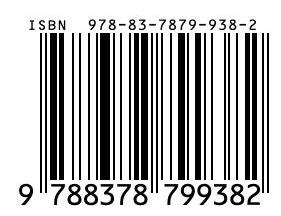
\includegraphics[max width=\textwidth, center]{2024_11_21_6574e892c2387ce90f12g-16}


\end{document}